\section*{Properties of IVPU game}
By dividing the characteristic function into two parts like $c(s)=c_0(s)+m(s)P, s \in S$

As a common practice, we can obtain the dual of $\omega(P)$:

\begin{equation}\label{dual}
 {\omega^*(P)}=\mathop{\max}_{\rho} \{c_0(V)+m(V)P+\sum_{s\in S\setminus\{V\}}-\rho_s[c_0(s)+m(s)P]:
 \sum_{s\in S\setminus\{V\}:k\in s}\rho_s=1,\forall k \in V,\rho_s\geq 0,\forall s \in S \setminus{V}\}
\end{equation}

Based on the above defined PSPF, we can establish Theorem 1 below, showing the property of this function.

\begin{thm}\label{thm1}
$\omega(P)$ is piecewise linear, and convex in price P at each sub-interval $[P_{i+1},P_{i}]$.
\end{thm}

In this situation, the interval size of price can be calculated when $t_i$ is known. And we can obtain that under what circumstances the machine number will change. We set the different intervals where the number of machines remain unchanged as $I_i$ respectively. The extreme points of these intervals are recorded as $P_i$ respectively, which represents the price when the number of using machine changes from $i$ to $i-1$. Specially, $P_1$ denotes the extreme point of the whole interval, which is the value of price or setup cost when using one machine and subsidy equals zero.

Note that the costs of all the exponential coalitions can be easily calculated by the SPT rules, we have Lemma \ref{lem1}.

\begin{lem}\label{lem1}

The breaking price,$P_i(2 \leq i \leq v)$, which is at the extreme points of the sub-intervals $I_i$ can be obtained by SPT rules in polynomial time.
\end{lem}

According to the above lemma \ref{lem1}, we can obtain all the extreme points of the sub-intervals, i.e., the number of using machines decreases by one when the price or setup cost equals $P_i$.

\begin{thm}\label{thm2}
Boundary price $P^*$ equals $\sum_{i=2}^v P_i$, and can be obtained in polynomial time.
\end{thm}

With Theorem \ref{thm2}, we obtain all the breakpoints during the interval of the price where the machine number changes and the subsidy is $0$. Then we'll focus on the specific property of subsidy.

\begin{thm}\label{thm3}
$\omega(P)$ can be bounded by zero when the number of machines used by $c(V,P)$ is larger than $\frac{v}{2}$.
\end{thm}

In other words, when the numbers of machine is larger than half of players, the grand coalition does't need any subsidy from the externality.

Lemma4 The sum of absolute values of slopes at both sides of $S_i$ is 1.

Define a new game, that is Single Machine Scheduling Game(SMSG)
\[
\begin{aligned}
c(s,P,'m='1) = & {\min} \sum_{k\in V}\sum_{j\in O} {c_{kj} x_{kj} + P} \\
{s.t.}\quad & \sum_{j \in O} x_{kj}-y_k^s=0, \forall k \in V, \\
& \sum_{k\in V} x_{kj} \leq 1, \forall j \in O,  \\
& x_{kj} \in \{0,1\} , \forall k \in V, \forall j \in O,\\
& y_k^s=1, k \in s, y_k^s=0, k \notin s.
\end{aligned}
\]

Define that
\[
  {\omega_1(P)}=\mathop{\min}_{\alpha}\{c(V,P)-\alpha(V): \alpha(s)\leq c(s,P,1), \forall s \in S, \alpha\in\mathbb{R}^{v}\},
\]

\begin{thm}\label{thm4}
For SMSG(or, MSG with only one machine), given $P \in [0, P^*]$ (or, $[P_2,P_1]$),
the range of each segments in the interval for function $\omega(P)$ is within $\left( -1 , -\frac{1}{n-1} \right]$, and the number of breakpoints for function $\omega(P)$ is within $ O(v^2) $.
\end{thm}

Until here, we described the main property of the whole figure.
And a diagram of the number of machines and subsidy on setup cost, with its essential features being showed below.

\begin{figure}[h]%%图
	\centering  %插入的图片居中表示
	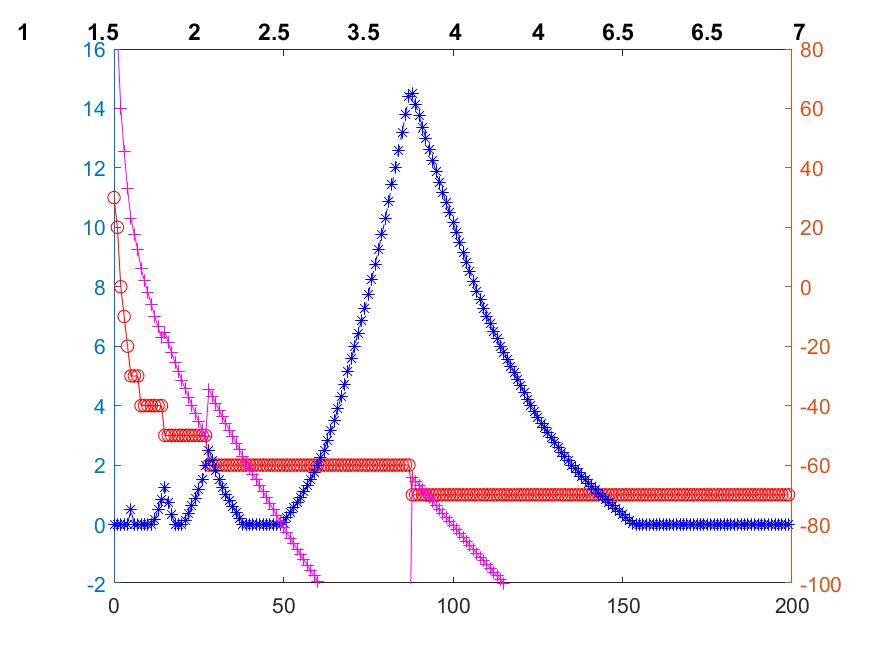
\includegraphics[width=0.8\linewidth]{Figures/Image30}  %插入的图,包括JPG,PNG,PDF,EPS等,放在源文件目录下
	\caption{The number of machines and subsidy on setup cost.}  %图片的名称
	\label{fig:Image11}   %标签,用作引用
\end{figure}

When the number of available machines $m$ is larger than $v$, the image is complete. And when the number of available machines $m$ is less than $v$, the image will be truncated.

The processing times of all players with the arrangement from small to large are listed on the top of this figure.
The red and blue lines stand for the machine number and subsidy, respectively.
The horizontal ordinate represents the price or setup cost.
The left ordinate represents the value of machine number,while the right represents the value of subsidy.

As the coalitional stability constraints showed above, the exponential inequality constraints are so tricky that we must figure out a method to simplify these constraints to obtain the optimal results. Fortunately for us, we find the Theorem \ref{thm5}.

\begin{thm}\label{thm5}
then the original problem $\omega(P)$ is equivalent to $\omega_1(P)$, which is polynomially solvable by cutting plane (see CP Algorithm below).

\end{thm}

By establishing the Theorem 5, we can design the specific algorithm to eliminate the redundant inequalitie, which will save us from the trouble of solving $c(s)$ and speed up the solution.
